% Appendix Template

\chapter{Il framework Torch} % Main appendix title
\label{AppendixB} % Change X to a consecutive letter; for referencing this appendix elsewhere, use \ref{AppendixX}
\def \path {Appendices/}
\section{Introduzione}
Torch\parencite{WTorch} è un framework per il calcolo numerico versatile che estende il linguaggio Lua. L'obiettivo è quello di fornire un ambiente flessibile per il progetto e addestramento di sistemi di machine learning anche su larga scala.\\
La flessibilità è ottenuta grazie a Lua stesso, un linguaggio di scripting estremamente leggero e efficiente. Le prestazioni sono garantite da backend compilati ed ottimizzati (C,C++,CUDA,OpenMP/SSE) per le routine di calcolo numerico di basso livello.
\\
\\
Gli obiettivi degli autori erano: (1) facilità di sviluppo di algoritmi numerici; (2) facilità di
estensione, incluso il supporto ad altre librerie; (3) la velocità.\\
Gli obiettivi (2) e (3) sono stati soddisfatti tramite l'utilizzo di Lua poiché un linguaggio interpretato risulta conveniente per il testing rapido in modo interattivo; garantisce facilità di sviluppo e, grazie alle ottime C-API, unisce in modo eterogeneo le varie librerie,
nascondendole sotto un'unica struttura di linguaggio di scripting.  Infine, essendo ossessionati dalla velocità, è stato scelto Lua poiché è un veloce linguaggio di scripting e può inoltre contare su un efficiente compilatore JIT.
Inoltre, Lua ha il grosso vantaggio di essere stato progettato per essere facilmente inserito nelle applicazioni scritte in C e consente quindi di “wrappare” le sottostanti implementazioni in C/C++ in maniera banale. Il binding C per il Lua è tra i più semplici e dona quindi grande estensibilità al progetto Torch. 
\\
\\
Torch è un framework auto-contenuto e estremamente portabile su ogni piattaforma: iOS, Android, FPGA, processori DSP ecc. Gli scrpt che vengono scritti per Torch riescono ad essere eseguiti su queste piattaforme senza nessuna modifica.
\\
Per soddisfare il requisito (1) hanno invece ideato un oggetto chiamato \texttt{'Tensor'}, il quale altro non è che una “vista” geometrica di una particolare area di memoria, e permette una efficiente e semplice 
gestione di vettori a N dimensioni, tensori appunto.\\
L’oggetto Tensor fornisce anche un’efficiente gestione della memoria: ogni operazione fatta su di esso non alloca nuova memoria, ma trasforma il tensore esistente o ritorna un nuovo tensore che referenzia la stessa area di memoria.
Torch fornisce un ricco set di routine di calcolo numerico: le comuni routine di Matlab, algebra lineare, convoluzioni, FFT, ecc. Ci sono molti package per diversi ambiti: Machine Learning, Visione Artificiale, Image \& Video Processing, Speech Recognition, ecc.\\
\\
I package più importanti per il machine learning sono: 
\begin{itemize}
\item \textbf{nn}: Neural Network, fornisce ogni sorta di modulo per la costruzione di reti neurali, reti neural profonde (deep), regressione lineare, MLP, autoencoders ecc. È il package utilizzato nel progetto. Per topologie di rete bleeding-edge si suggerisce il package \textbf{'nnx'}; 
\item  \textbf{optim}: package per l'ottimizzazione della discesa del gradiente  Fondamentale per avere buone performance nel training della rete; 
\item \textbf{unsup}: è un toolbox per l'apprendimento non supervisionato; 

\item \textbf{Image}: contiene tutte le funzioni atte all'image processing; 

\item \textbf{cunn}: package per utilizzare le reti neurali sfruttando la potenza di calcolo parallelo delle GPU, mediante l'architettura CUDA. 
\end{itemize}
L'architettura del framework è raffigurata in figura \ref{fig:torch}.\\

\begin{figure}[h!]
 \centering
 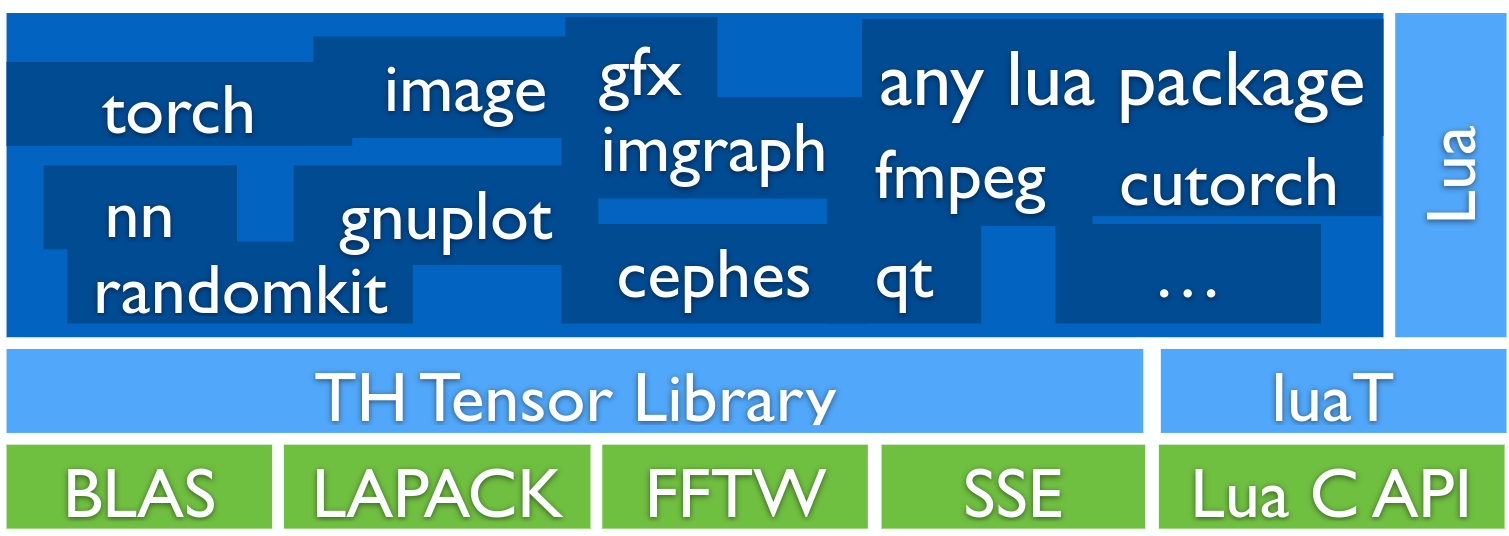
\includegraphics[width=1.0\textwidth]{\path/torch.png} 
 \caption{Architettura del framework Torch}
 \label{fig:torch}
\end{figure}
\\
Torch è adottato da una fiorente comunità attiva di ricercatori in diverse università e importanti centri di ricerca come quelli di IBM; il dipartimento di IA di Facebook (FAIR); Google DeepMind prima di passare a TensorFlow nel 2016.

\section{Utilizzo base per reti neurali}
Costruire modelli di reti neurali è una procedura rapida con Torch, ecco alcuni esempi: 
\begin{lstlisting}[language={[5.2]Lua}]
------------------------------------------------------------
-- simple linear model: logistic regression
------------------------------------------------------------
model:add(nn.Reshape(3*32*32))
model:add(nn.Linear(3*32*32,#classes))

------------------------------------------------------------
-- classic 2-layer fully-connected MLP
------------------------------------------------------------
model:add(nn.Reshape(3*32*32))
model:add(nn.Linear(3*32*32, 1*32*32))
model:add(nn.ReLU())
model:add(nn.Linear(1*32*32, #classes))

------------------------------------------------------------
-- convolutional layer
------------------------------------------------------------
--hyper-parameters
nfeats = 3 --3D input volume
nstates = {16, 64, 128} --output at each level
filtsize = 5 --filter size or kernel 
poolsize = 2

--Here's only the first stage. 
--The others look the same except for the nstates you're gonna use

-- filter bank -> squashing -> max pooling
model:add(nn.SpatialConvolutionMM(nfeats, nstates[1], filtsize, filtsize))
model:add(nn.ReLU())
model:add(nn.SpatialMaxPooling(poolsize, poolsize, poolsize, poolsize))
\end{lstlisting}
\subsection{Supporto CUDA}
CUDA (Compute Unified Device Architecture) è l'architettura di elaborazione in parallelo di NVIDIA che permette netti aumenti delle prestazioni di computing grazie allo sfruttamento della potenza di calcolo delle GPU per operazioni “general purpose”.\\
Torch offre un package chiamato \texttt{'cunn'} per usufruire di CUDA. Il package è basato su un tensore chiamato \texttt{'torch.CudaTensor()'} che altro non è che un normale Tensor che risiede ed utilizza la memoria della DRAM della GPU; tutte le operazioni definite per l'oggetto Tensor sono definite normalmente anche per il CudaTensor, il quale astrae completamente dall'utilizzo della GPU, offrendo un'interfaccia semplice e permettendo di sfruttare gli stessi script che si usano per l'elaborazione CPU. L'unica modifica da apportare, quindi, è cambiare il tipo di tensore. 
\begin{lstlisting}[language={[5.2]Lua}]
tf = torch.FloatTensor(4,100,100) -- CPU's DRAM
tc = tf:cuda() -- GPU's DRAM 
tc:mul() -- run on GPU
res = tc:float() -- res is instantiated on CPU's DRAM

--similarly, after we've built our model
--we can move it to the GPU by doing
model:cuda()
--we also need to compute our loss on GPU
criterion:cuda()

--now we're set, we can train our model on the GPU 
--just by following the standard training procedure seen in (Capitolo 4)
\end{lstlisting}


\section{ResNet}
Una rappresentazione testuale del modello a 18 strati di Residual Network. 

\begin{lstlisting}[language={[5.2]Lua}]
nn.Sequential {
  [input -> (1) -> (2) -> (3) -> (4) -> (5) -> (6) -> (7) -> (8) -> (9) -> output]
  (1): cudnn.SpatialConvolution(3 -> 16, 3x3, 1,1, 1,1) without bias
  (2): nn.SpatialBatchNormalization (4D) (16)
  (3): cudnn.ReLU
  (4): nn.Sequential {
    [input -> (1) -> (2) -> (3) -> output]
    (1): nn.Sequential {
      [input -> (1) -> (2) -> (3) -> output]
      (1): nn.ConcatTable {
        input
          |`-> (1): nn.Sequential {
          |      [input -> (1) -> (2) -> (3) -> (4) -> (5) -> output]
          |      (1): cudnn.SpatialConvolution(16 -> 16, 3x3, 1,1, 1,1) without bias
          |      (2): nn.SpatialBatchNormalization (4D) (16)
          |      (3): cudnn.ReLU
          |      (4): cudnn.SpatialConvolution(16 -> 16, 3x3, 1,1, 1,1) without bias
          |      (5): nn.SpatialBatchNormalization (4D) (16)
          |    }
           `-> (2): nn.Identity
           ... -> output
      }
      (2): nn.CAddTable
      (3): cudnn.ReLU
    }
    (2): nn.Sequential {
      [input -> (1) -> (2) -> (3) -> output]
      (1): nn.ConcatTable {
        input
          |`-> (1): nn.Sequential {
          |      [input -> (1) -> (2) -> (3) -> (4) -> (5) -> output]
          |      (1): cudnn.SpatialConvolution(16 -> 16, 3x3, 1,1, 1,1) without bias
          |      (2): nn.SpatialBatchNormalization (4D) (16)
          |      (3): cudnn.ReLU
          |      (4): cudnn.SpatialConvolution(16 -> 16, 3x3, 1,1, 1,1) without bias
          |      (5): nn.SpatialBatchNormalization (4D) (16)
          |    }
           `-> (2): nn.Identity
           ... -> output
      }
      (2): nn.CAddTable
      (3): cudnn.ReLU
    }
    (3): nn.Sequential {
      [input -> (1) -> (2) -> (3) -> output]
      (1): nn.ConcatTable {
        input
          |`-> (1): nn.Sequential {
          |      [input -> (1) -> (2) -> (3) -> (4) -> (5) -> output]
          |      (1): cudnn.SpatialConvolution(16 -> 16, 3x3, 1,1, 1,1) without bias
          |      (2): nn.SpatialBatchNormalization (4D) (16)
          |      (3): cudnn.ReLU
          |      (4): cudnn.SpatialConvolution(16 -> 16, 3x3, 1,1, 1,1) without bias
          |      (5): nn.SpatialBatchNormalization (4D) (16)
          |    }
           `-> (2): nn.Identity
           ... -> output
      }
      (2): nn.CAddTable
      (3): cudnn.ReLU
    }
  }
  (5): nn.Sequential {
    [input -> (1) -> (2) -> (3) -> output]
    (1): nn.Sequential {
      [input -> (1) -> (2) -> (3) -> output]
      (1): nn.ConcatTable {
        input
          |`-> (1): nn.Sequential {
          |      [input -> (1) -> (2) -> (3) -> (4) -> (5) -> output]
          |      (1): cudnn.SpatialConvolution(16 -> 32, 3x3, 2,2, 1,1) without bias
          |      (2): nn.SpatialBatchNormalization (4D) (32)
          |      (3): cudnn.ReLU
          |      (4): cudnn.SpatialConvolution(32 -> 32, 3x3, 1,1, 1,1) without bias
          |      (5): nn.SpatialBatchNormalization (4D) (32)
          |    }
           `-> (2): nn.Sequential {
                 [input -> (1) -> (2) -> output]
                 (1): nn.SpatialAveragePooling(1x1, 2,2)
                 (2): nn.Concat {
                   input
                     |`-> (1): nn.Identity
                      `-> (2): nn.MulConstant
                      ... -> output
                 }
               }
           ... -> output
      }
      (2): nn.CAddTable
      (3): cudnn.ReLU
    }
    (2): nn.Sequential {
      [input -> (1) -> (2) -> (3) -> output]
      (1): nn.ConcatTable {
        input
          |`-> (1): nn.Sequential {
          |      [input -> (1) -> (2) -> (3) -> (4) -> (5) -> output]
          |      (1): cudnn.SpatialConvolution(32 -> 32, 3x3, 1,1, 1,1) without bias
          |      (2): nn.SpatialBatchNormalization (4D) (32)
          |      (3): cudnn.ReLU
          |      (4): cudnn.SpatialConvolution(32 -> 32, 3x3, 1,1, 1,1) without bias
          |      (5): nn.SpatialBatchNormalization (4D) (32)
          |    }
           `-> (2): nn.Identity
           ... -> output
      }
      (2): nn.CAddTable
      (3): cudnn.ReLU
    }
    (3): nn.Sequential {
      [input -> (1) -> (2) -> (3) -> output]
      (1): nn.ConcatTable {
        input
          |`-> (1): nn.Sequential {
          |      [input -> (1) -> (2) -> (3) -> (4) -> (5) -> output]
          |      (1): cudnn.SpatialConvolution(32 -> 32, 3x3, 1,1, 1,1) without bias
          |      (2): nn.SpatialBatchNormalization (4D) (32)
          |      (3): cudnn.ReLU
          |      (4): cudnn.SpatialConvolution(32 -> 32, 3x3, 1,1, 1,1) without bias
          |      (5): nn.SpatialBatchNormalization (4D) (32)
          |    }
           `-> (2): nn.Identity
           ... -> output
      }
      (2): nn.CAddTable
      (3): cudnn.ReLU
    }
  }
  (6): nn.Sequential {
    [input -> (1) -> (2) -> (3) -> output]
    (1): nn.Sequential {
      [input -> (1) -> (2) -> (3) -> output]
      (1): nn.ConcatTable {
        input
          |`-> (1): nn.Sequential {
          |      [input -> (1) -> (2) -> (3) -> (4) -> (5) -> output]
          |      (1): cudnn.SpatialConvolution(32 -> 64, 3x3, 2,2, 1,1) without bias
          |      (2): nn.SpatialBatchNormalization (4D) (64)
          |      (3): cudnn.ReLU
          |      (4): cudnn.SpatialConvolution(64 -> 64, 3x3, 1,1, 1,1) without bias
          |      (5): nn.SpatialBatchNormalization (4D) (64)
          |    }
           `-> (2): nn.Sequential {
                 [input -> (1) -> (2) -> output]
                 (1): nn.SpatialAveragePooling(1x1, 2,2)
                 (2): nn.Concat {
                   input
                     |`-> (1): nn.Identity
                      `-> (2): nn.MulConstant
                      ... -> output
                 }
               }
           ... -> output
      }
      (2): nn.CAddTable
      (3): cudnn.ReLU
    }
    (2): nn.Sequential {
      [input -> (1) -> (2) -> (3) -> output]
      (1): nn.ConcatTable {
        input
          |`-> (1): nn.Sequential {
          |      [input -> (1) -> (2) -> (3) -> (4) -> (5) -> output]
          |      (1): cudnn.SpatialConvolution(64 -> 64, 3x3, 1,1, 1,1) without bias
          |      (2): nn.SpatialBatchNormalization (4D) (64)
          |      (3): cudnn.ReLU
          |      (4): cudnn.SpatialConvolution(64 -> 64, 3x3, 1,1, 1,1) without bias
          |      (5): nn.SpatialBatchNormalization (4D) (64)
          |    }
           `-> (2): nn.Identity
           ... -> output
      }
      (2): nn.CAddTable
      (3): cudnn.ReLU
    }
    (3): nn.Sequential {
      [input -> (1) -> (2) -> (3) -> output]
      (1): nn.ConcatTable {
        input
          |`-> (1): nn.Sequential {
          |      [input -> (1) -> (2) -> (3) -> (4) -> (5) -> output]
          |      (1): cudnn.SpatialConvolution(64 -> 64, 3x3, 1,1, 1,1) without bias
          |      (2): nn.SpatialBatchNormalization (4D) (64)
          |      (3): cudnn.ReLU
          |      (4): cudnn.SpatialConvolution(64 -> 64, 3x3, 1,1, 1,1) without bias
          |      (5): nn.SpatialBatchNormalization (4D) (64)
          |    }
           `-> (2): nn.Identity
           ... -> output
      }
      (2): nn.CAddTable
      (3): cudnn.ReLU
    }
  }
  (7): cudnn.SpatialAveragePooling(8x8, 1,1)
  (8): nn.View(64)
  (9): nn.Linear(64 -> 10)
}

\end{lstlisting}